\begin{frame}[fragile]{Empirical Evaluation}
  \begin{block}{Research Questions}
    \begin{itemize}
        \item Does \acrshort{dpbt} generate incremental results regardless of the size of the graph?
        \item Does the type of query $Q$ impact on the execution of \acrshort{dpbt}?
        \item How effectively \acrshort{dpbt} implements a \emph{pay-as-you-go} model?
        \item Does \acrshort{dpbt} handle memory and threads efficiently?
    \end{itemize}        
  \end{block}
\end{frame}

\begin{frame}[fragile]{Empirical Evaluation}
  \begin{block}{Research Questions}
    \begin{itemize}
        \item Does \acrshort{dpbt} generate incremental results regardless of the size of the graph?
        \item Does the type of query $Q$ impact on the execution of \acrshort{dpbt}?
        \item How effectively \acrshort{dpbt} implements a \emph{pay-as-you-go} model?
        \item Does \acrshort{dpbt} handle memory and threads efficiently?
    \end{itemize}        
  \end{block}
  \begin{block}{Experiments}
    \begin{itemize}
      \item \textbf{Continuous behavior Analysis}: using \acrshort{dt} and \acrshort{dk} to assess the continuous behavior capabilities.
      \item \textbf{Benchmark Analysis}: to identify how the behavior of \acrshort{dpbt} varies depending on the type of query command.
      \item \textbf{Performance Analysis} \acrfull{ghc} Profiling for one of the graphs to measure multithreading and memory allocation. 
    \end{itemize}
  \end{block}
\end{frame}

\begin{frame}[fragile]{Experiment Configuration}
  \begin{block}{Graphs Tested}
    \begin{table}[H]
      \centering
      \resizebox{1\textwidth}{!}{
      \begin{tabular}{|p{0.25\linewidth}|c|c|c|c|c|}
        \hline
       \textbf{Network} & \textbf{$|U|$} & \textbf{$|L|$} & \textbf{$|E|$} & \textbf{Wedges} & \textbf{\#\acrshort{bt}} \\
       \hline
       Dbpedia & 18422 & 168338 & 233286 & $1.45 \times 10^8$ & $3.62 \times 10^8$\\
       \hline
       Moreno Crime & 829 & 551 & 1476 & 4816 & 211\\
       \hline
       Opsahl UC Forum  & 899 & 522 & 33720 & 174069 & $2.2 \times 10^7$ \\
       \hline
       Wang Amazon & 26112 & 799 & 29062 & $3.4 \times 10^6$ & 110269\\
       \hline
      \end{tabular}
      }
     \end{table}
  \end{block}
  \begin{block}{Hardware Environment}
    \begin{itemize}
          \item \emph{HPC Cluster at UPC}
          \item $x86$ $64$ bits
          \item $24$-Core Intel(R) Xeon(R) CPU X5650 processor of $2.67$ GHz
          \item \emph{Hyper-threading} enable
          \item $40 GB$ up to $120 GB$ of RAM for the biggest \acrfull{dbpedia} graph
      \end{itemize}        
  \end{block}
\end{frame}

\begin{frame}[fragile]{Experiment Configuration}
  \begin{block}{Test Case Scenarios}
    \begin{table}[H]
      \centering
      \resizebox{1\textwidth}{!}{
        \begin{tabular}{|l|c|c|}
          \hline
          \textbf{Scenario ID} & \textbf{Name} & \textbf{Search by}\\
          \hline
          E-H & Edge High & edge with high incidence \\
          \hline
          E-L & Edge Low & edge with low incidence \\
          \hline
          E-M & Edge Medium & edge with medium incidence \\
          \hline
          VL-H & $l \in L$ High & vertex in lower layer with high incidence \\
          \hline
          VL-L & $l \in L$ Low & vertex in lower layer with low incidence \\
          \hline
          VL-M & $l \in L$ Medium & vertex in lower layer with medium incidence \\
          \hline
          VU-H & $u \in U$ High & vertex in upper layer with high incidence \\
          \hline
          VU-L & $u \in U$ Low & vertex in upper layer with low incidence \\
          \hline
          VU-M & $u \in U$ Medium & vertex in upper layer with medium incidence \\
          \hline
        \end{tabular}
    }
     \end{table}
  \end{block}
\end{frame}

\begin{frame}[fragile]{Experiment Configuration}
  \begin{block}{Selection of Query $Q$ values}
    \begin{itemize}
      \item Sort the vertices by its degree.
      \item Randomly select following a uniform distribution,  a vertex or edge depending on the scenario, from the subset of vertices or edges with the required incidence.
      \item Execution of a sample of experiments to check if that selections provides results or not. If not, the test case is eliminated.
    \end{itemize}    
  \end{block}
\end{frame}


\begin{frame}[fragile]{E1: Continuous Behavior: \acrshort{dt} and \acrshort{dk}}
  \begin{figure}[!htp]
    \centering
    \begin{subfigure}[t]{0.45\textwidth}
     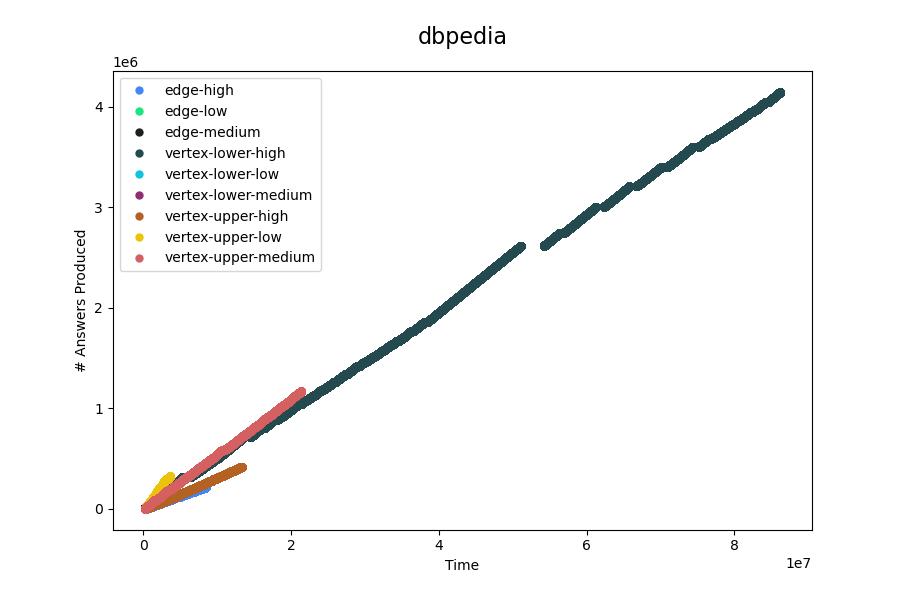
\includegraphics[width=1\linewidth, height=0.4\textheight]{experiments/diepfy/dbpedia.png}
    \end{subfigure}\hfill
    \begin{subfigure}[t]{0.45\textwidth}
     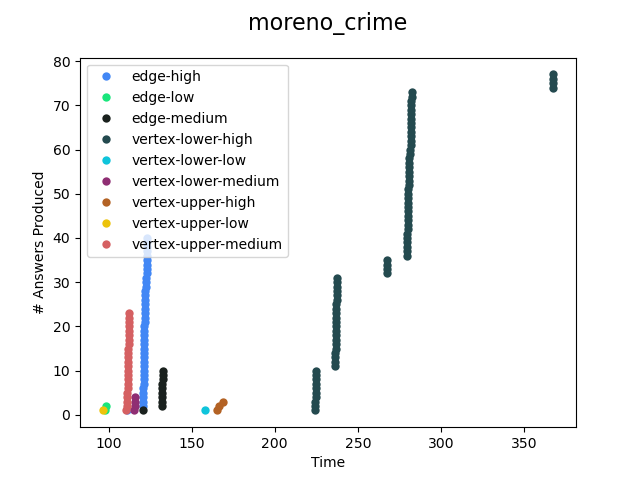
\includegraphics[width=1\linewidth, height=0.4\textheight]{experiments/diepfy/moreno_crime.png}
    \end{subfigure}
    \vspace{0.5cm}
  
    \begin{subfigure}[t]{0.45\textwidth}
     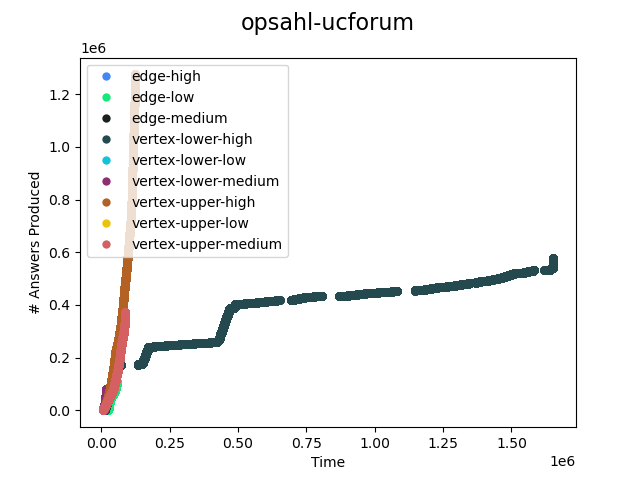
\includegraphics[width=1\linewidth, height=0.4\textheight]{experiments/diepfy/opsahl-ucforum.png}
    \end{subfigure}\hfill
    \begin{subfigure}[t]{0.45\textwidth}
      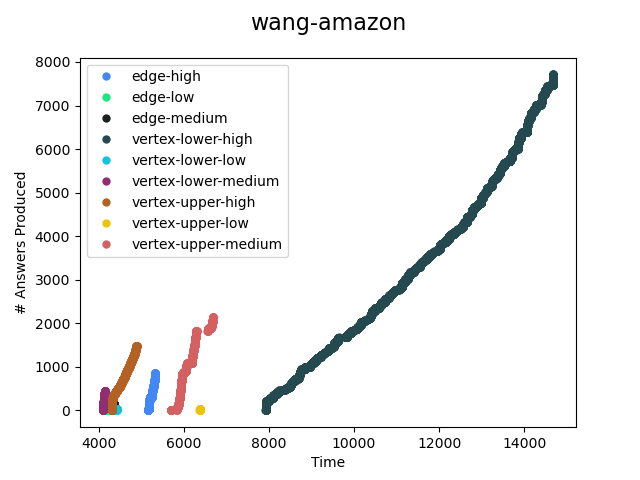
\includegraphics[width=1\linewidth, height=0.4\textheight]{experiments/diepfy/wang-amazon.png}
     \end{subfigure}
   \end{figure}
  \end{frame}

  \begin{frame}[fragile]{E1: Continuous Behavior: \acrshort{dt} and \acrshort{dk}}
    \begin{figure}[!htp]
      \centering
      \begin{subfigure}[t]{0.45\textwidth}
      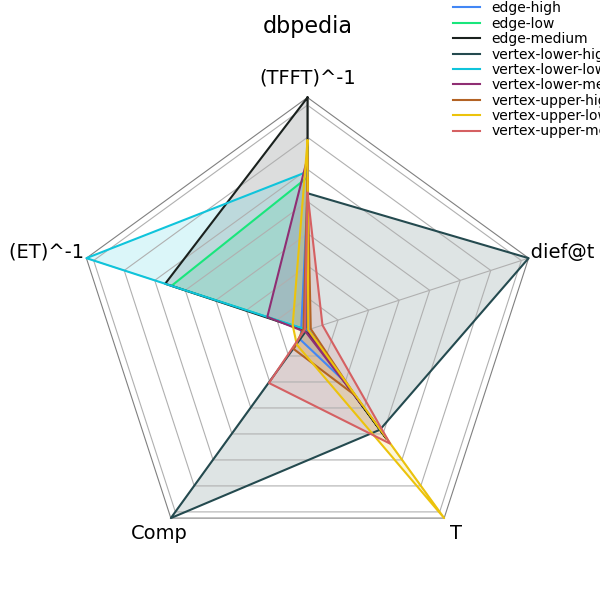
\includegraphics[width=1\linewidth, height=0.4\textheight]{experiments/diepfy/dbpedia_radial.png}
      \end{subfigure}\hfill
      \begin{subfigure}[t]{0.45\textwidth}
      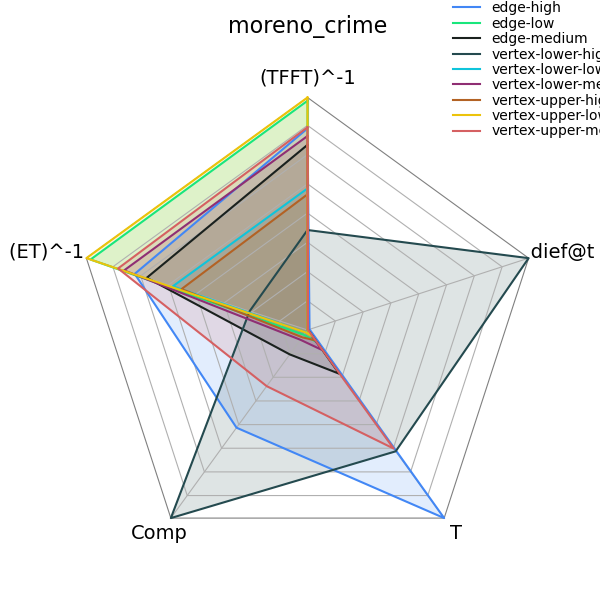
\includegraphics[width=1\linewidth, height=0.4\textheight]{experiments/diepfy/moreno_crime_radial.png}
      \end{subfigure}
      \vspace{0.5cm}
      %
      \begin{subfigure}[t]{0.45\textwidth}
      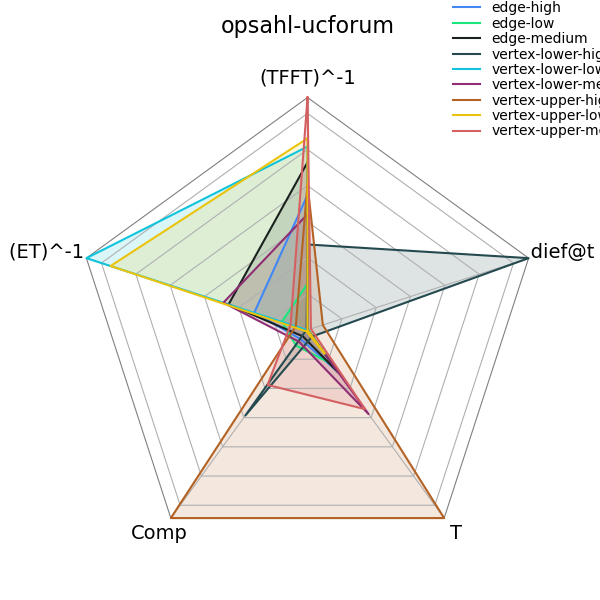
\includegraphics[width=1\linewidth, height=0.4\textheight]{experiments/diepfy/opsahl-ucforum_radial.png}
      \end{subfigure}\hfill
      \begin{subfigure}[t]{0.45\textwidth}
        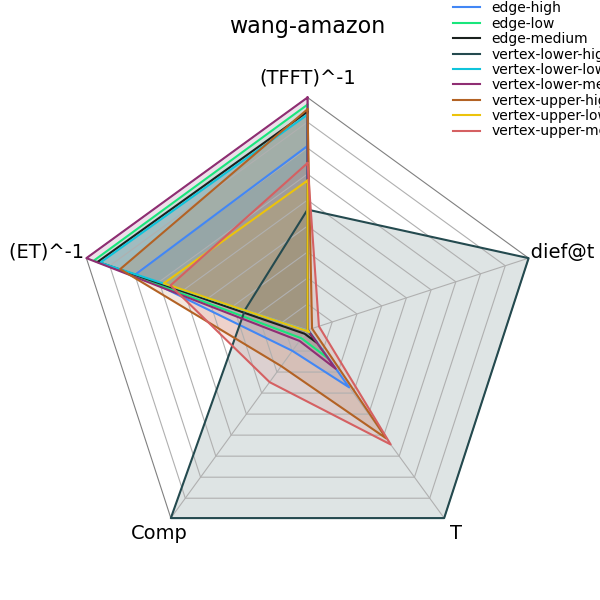
\includegraphics[width=1\linewidth, height=0.4\textheight]{experiments/diepfy/wang-amazon_radial.png}
      \end{subfigure}
    \end{figure}
    \end{frame}

  \begin{frame}[fragile]{E1: Continuous Behavior: \acrshort{dt} and \acrshort{dk}}
    \begin{table}[H]
      \centering
      \resizebox{1\textwidth}{!}{
      \begin{tabular}{|p{0.25\linewidth}|c|c|c|}
        \hline
       \textbf{Network} & \textbf{Scenario ID} & \textbf{\acrshort{dt} Metric}  & \textbf{\acrshort{dk} Metric}\\
       \hline
       \multirow{3}{*}{Moreno Crime}
        & \cellcolor{yellow!35}VU-H & \cellcolor{yellow!35}$6.05 \times 10^2$ & $0.00$\\
        & \cellcolor{blue!25}VL-H & \cellcolor{blue!25}$7.95 \times 10^3$ & $0.00$\\
        & \cellcolor{blue!25}E-H & \cellcolor{blue!25}$9.85 \times 10^3$ & $0.00$\\
        \hline
        \multirow{3}{*}{Dbpedia}
        & \cellcolor{yellow!35}VU-H & \cellcolor{yellow!35}$3.32 \times 10^{13}$ & $1.97 \times 10^5$\\
        & \cellcolor{blue!25}VL-H &  \cellcolor{blue!25}$1.81 \times 10^{14}$ & $2.34 \times 10^4$\\
        & \cellcolor{blue!25}E-H &  \cellcolor{blue!25}$1.75 \times 10^{13}$ & $3.28 \times 10^5$\\
        \hline
        \multirow{3}{*}{Opsahl UC Forum}
        & \cellcolor{blue!25}VU-H &  \cellcolor{blue!25}$1.99 \times 10^{12}$ & $1.27 \times 10^5$\\
        & \cellcolor{blue!25}VL-H &  \cellcolor{blue!25}$6.44 \times 10^{11}$ & $1.90 \times 10^5$\\
        & \cellcolor{yellow!35}E-H &  \cellcolor{yellow!35}$1.02 \times 10^{11}$ & $2.93 \times 10^5$\\
        \hline
        \multirow{3}{*}{Wang Amazon}
        & \cellcolor{yellow!35}VU-H & \cellcolor{yellow!35}$1.50 \times 10^7$ & $43.6$\\
        & \cellcolor{blue!25}VL-H & \cellcolor{blue!25}$2.24 \times 10^7$ & $63.1$\\
        & \cellcolor{blue!25}E-H & \cellcolor{blue!25}$8.06 \times 10^6$  & $42.3$\\
        \hline
      \end{tabular}
      }
     \end{table}
\end{frame}

\begin{frame}[fragile]{E2: Average Excution Time}
\begin{figure}[H]
  \begin{center}
     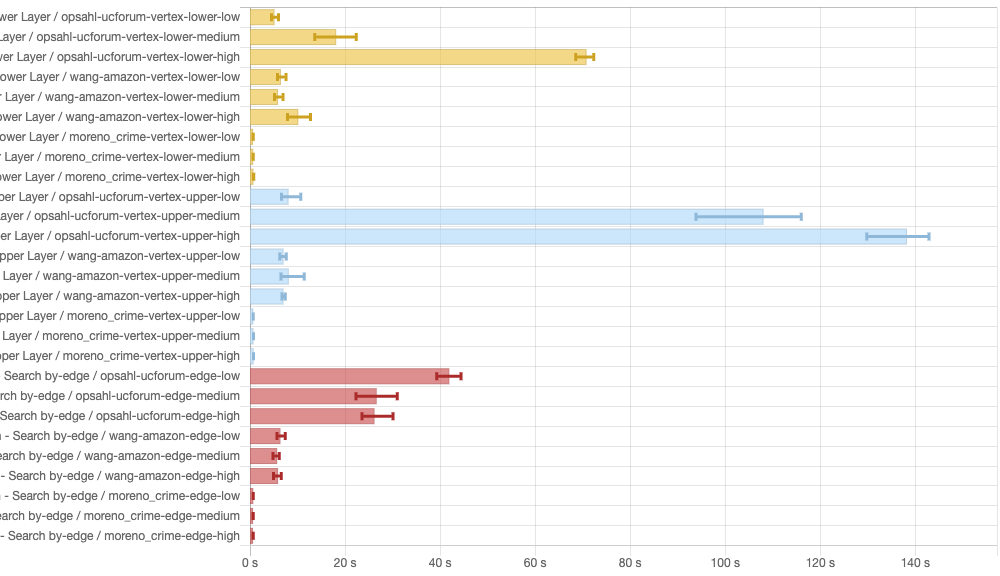
\includegraphics[width=1\textwidth]{experiments/bench_1}
  \end{center}
 \end{figure}
\end{frame}

\begin{frame}[fragile]{E2: Total Excution Time}
  \begin{figure}[H]
    \begin{center}
       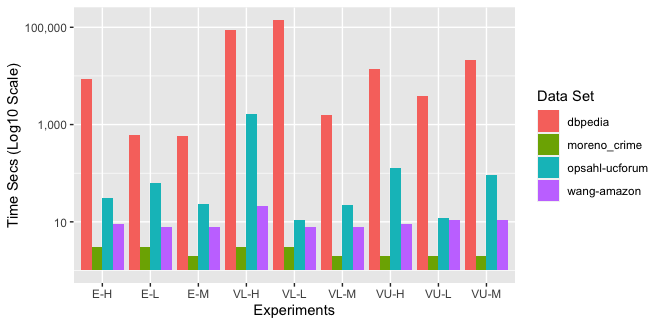
\includegraphics[width=1\textwidth] {experiments/execution_time_by_experiments}
    \end{center}
  \end{figure}
\end{frame}

\begin{frame}[fragile]{E3: Performance Analysis - Multithreading}
  \begin{figure}[H]
    \begin{center}
      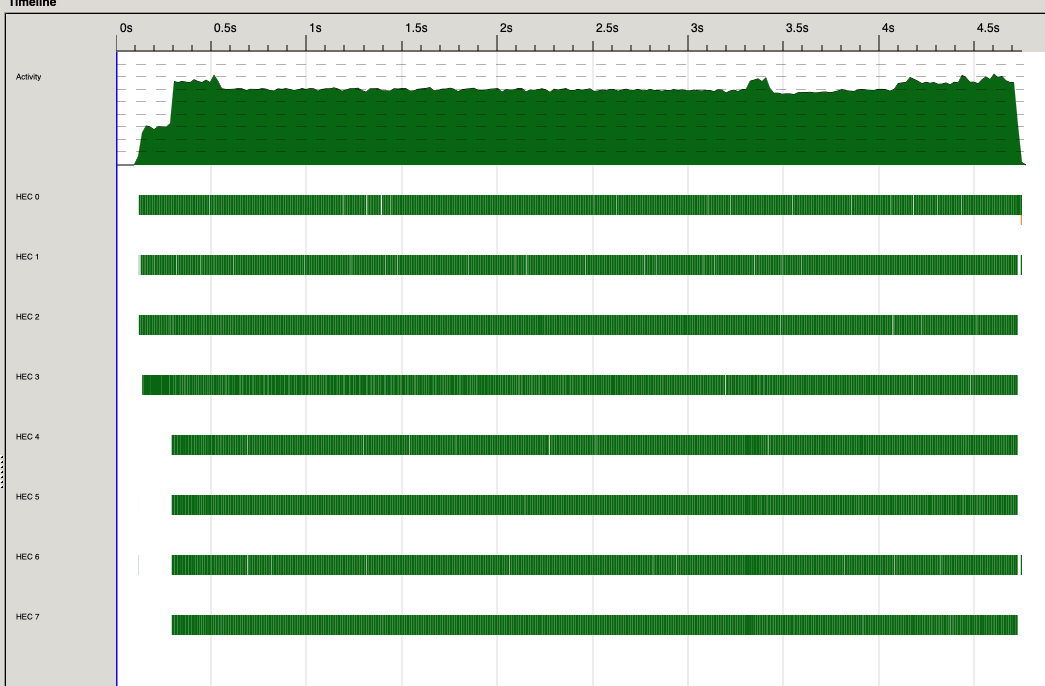
\includegraphics[width=1\textwidth]{experiments/thread/general_overview}
    \end{center}
  \end{figure}
\end{frame}

\begin{frame}[fragile]{E3: Performance Analysis - Memory Allocation}
  \begin{figure}[H]
    \begin{center}
      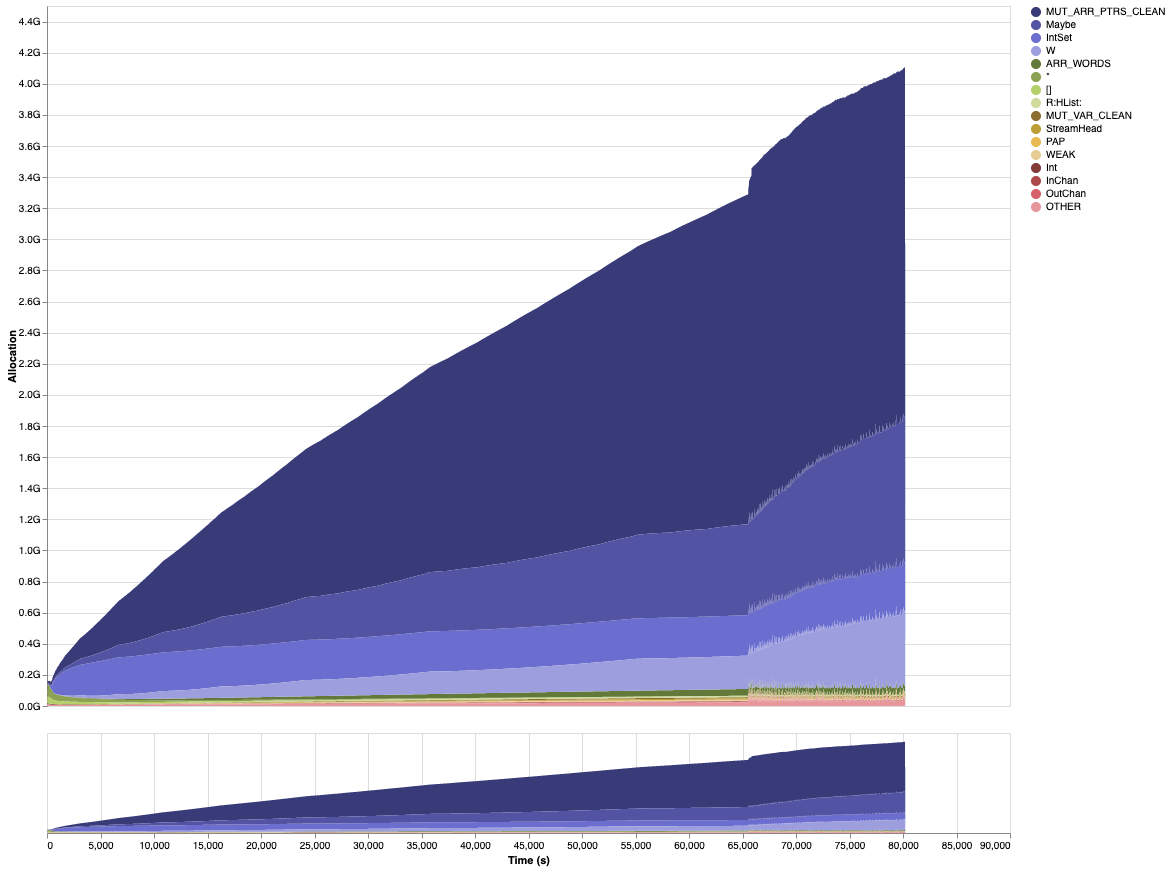
\includegraphics[width=0.8\textwidth] {experiments/mem/overview}
    \end{center}
  \end{figure}
\end{frame}


\begin{frame}[fragile]{Empirical Evaluation}
  \begin{block}{Conclusions}
    \begin{itemize}
      \item High values of the metric dief\@t indicates continuous behavior.
      \item Lower values of the metric dief\@k indicates continuous behavior.
      \item High values of the metrics \emph{Average Running Time} and \emph{Total Running Time} for scenarios which enumerates more bitriangles, are suggesting an effective implementation of a \emph{pay-as-you-go} model of \acrshort{dpbt}.
      \item Results captured by the \texttt{ThreadScope} tool indicating an even distribution of the threads among processors, showing efficient use of the parallel model.
      \item Results gathered by the \texttt{eventlog2html} tool suggesting that memory consumption is efficiently handled in the intermediate objects that \acrshort{dpfh}.
    \end{itemize} 
  \end{block}
\end{frame}
